\chapter{\texorpdfstring{$ 2^K $}{2K} Factorial Experiments}
\section{Designing \texorpdfstring{$ 2^K $}{2K} Factorial Experiments}
\makeheading{Week 9}
\begin{itemize}[*]
    \item $ 2^K $ factorial experiments involved $ K $ design factors, each at two levels.
\end{itemize}
\begin{itemize}
    \item These experiments are typically used for factor screening.
          \begin{itemize}[$\rightarrow$]
              \item \textbf{Primary Goal}: Determine which among the $ K $ factors significantly influence the response variable.
              \item \textbf{Secondary Goal}: Determine which combination of levels is optimal.
                    \begin{itemize}[$\hookrightarrow$]
                        \item This is only relevant if the levels experimented with are the only ones of interest.
                    \end{itemize}
          \end{itemize}
\end{itemize}
\begin{itemize}[$\rightarrow$]
    \item The design of the experiment involves:
          \begin{enumerate}[1.]
              \item Choose the MOI and response variables.
                    \begin{itemize}[$\hookrightarrow$]
                        \item Dictated by the question.
                    \end{itemize}
              \item Choose the design factors.
                    \begin{itemize}[$\hookrightarrow$]
                        \item Choose $ K $ factors that may influence the response and that you want to learn about.
                    \end{itemize}
              \item Choose the levels of the design factors.
                    \begin{itemize}[$\hookrightarrow$]
                        \item With the goal of factor screening we want to give influential factors as
                              an opportunity as possible to show themselves as being influential.
                        \item Pick levels that are quite different. For example, colour and discount amount.
                    \end{itemize}
              \item Define experimental conditions.
                    \begin{itemize}[$\hookrightarrow$]
                        \item These are the $ 2^K $ unique combinations of the $ K $ factors' levels.
                    \end{itemize}
              \item Assign $ n $ experimental units to each condition.
                    \begin{itemize}[$\hookrightarrow$]
                        \item Balance is not necessary, it's just notationally convenient.
                        \item Overall sample size: $ N=n2^K $.
                    \end{itemize}
          \end{enumerate}
\end{itemize}
\begin{itemize}
    \item In two-level experiments we regard the two levels of a factor as \emph{low} and \emph{high} values of that factor.
          \begin{itemize}
              \item If a factor is categorical, then ``low'' vs. ``high'' labelling is arbitrary.
          \end{itemize}
    \item We represent each factor by a binary variable:
          \[ x=\begin{cases*}
                  -1 & if the factor is at its ``low'' level  \\
                  1  & if the factor is at its ``high'' level
              \end{cases*} \]
          \begin{itemize}[*]
              \item We \underline{could} alternatively code each $ x $ as an indicator variable, but the $ \pm 1 $ coding
                    gives rise to some convenient statistical properties.
          \end{itemize}
\end{itemize}
\begin{itemize}[$\rightarrow$]
    \item With the factor levels coded in this way, each experimental condition can be identified by a unique
          combination of plus and minus ones.
\end{itemize}
\begin{itemize}
    \item The experimental design can be completely summarized by the \textbf{design matrix}.
          \begin{itemize}
              \item $ 2^K $ rows (for each condition) and $ K $ columns (for each factor) of plus and minus ones.
          \end{itemize}
          \begin{itemize}[$\rightarrow$]
              \item The $ \pm 1 $ entries are organized such that each row corresponds to a unique condition and the
                    columns correspond to each of the factors.
              \item The design matrix provides a prescription for running the $2^K$ factorial experiment.
          \end{itemize}
\end{itemize}
\begin{Example}{$ 2^1 $ Design Matrix}{}
    \[ \begin{matrix}
            C1\rightarrow \\
            C2\rightarrow
        \end{matrix}\begin{bmatrix}
            -1 \\
            +1
        \end{bmatrix}=\begin{bmatrix}
            \Vector{x}_1
        \end{bmatrix} \]
\end{Example}
\begin{Example}{$ 2^2 $ Design Matrix}{}
    \[ \begin{matrix}
            C1\rightarrow \\
            C2\rightarrow \\
            C3\rightarrow \\
            C4\rightarrow
        \end{matrix}\begin{bmatrix}
            -1 & -1 \\
            +1 & -1 \\
            -1 & +1 \\
            +1 & +1
        \end{bmatrix}=\begin{bmatrix}
            \Vector{x}_1 & \Vector{x}_2
        \end{bmatrix} \]
\end{Example}
\begin{Example}{$ 2^3 $ Design Matrix}{}
    \[ \begin{matrix}
            C1\rightarrow \\
            C2\rightarrow \\
            C3\rightarrow \\
            C4\rightarrow \\
            C5\rightarrow \\
            C6\rightarrow \\
            C7\rightarrow \\
            C8\rightarrow
        \end{matrix}\begin{bmatrix}
            -1 & -1 & -1 \\
            +1 & -1 & -1 \\
            -1 & +1 & -1 \\
            +1 & +1 & -1 \\
            -1 & -1 & +1 \\
            +1 & -1 & +1 \\
            -1 & +1 & +1 \\
            +1 & -1 & +1
        \end{bmatrix}=\begin{bmatrix}
            \Vector{x}_1 & \Vector{x}_2 & \Vector{x}_3
        \end{bmatrix} \]
\end{Example}
\begin{itemize}[$\rightarrow$]
    \item $ 2^K $ experiments may also be visualized geometrically as $ K $-dimensional hypercubes.
          \begin{itemize}
              \item Vertices correspond to the unique configurations of the $ K $ factors' levels,
                    and hence experimental conditions.
                    \begin{itemize}[label={}]
                        \item \underline{Design Space}: the space of all possible combinations of the design factors' values.
                    \end{itemize}
          \end{itemize}
\end{itemize}
\section{Analyzing \texorpdfstring{$ 2^K $}{2K} Factorial Experiments}
\begin{itemize}
    \item Primary goal of a $2^K$ factorial experiment is factor screening.
          \begin{itemize}
              \item Interest lies primarily in estimation of main and interaction effects.
          \end{itemize}
\end{itemize}
\begin{itemize}[*]
    \item The \textbf{main effect} of a factor is defined as the expected change in response produced by changing that factor from
          its low to its high level.
    \item The \textbf{interaction effect} between two factors quantifies the difference between the main effect of one
          factor at the two levels of the other.
\end{itemize}
\subsection{An Intuition-Based Analysis}
\begin{Example}{Toy Example}{toy_ex}
    Factors A and B are investigated in a $ 2^2 $ factorial experiment with $ n=3 $.
    \begin{center}
        \begin{NiceTabular}{ccc|cc}
            \toprule
            Condition & Factor A & Factor B & Response ($ y $) & Average Response ($ \bar{y} $)\\
            \midrule
            1 & $ -1 $ & $ -1 $ & $ \Set{1,1,2} $ & $ 4/3 $\\
            2 & $ +1 $ & $ -1 $ & $ \Set{3,4,5} $ & $ 12/3 $\\
            3 & $ -1 $ & $ +1 $ & $ \Set{2,1,3} $ & $ 6/3 $\\
            4 & $ +1 $ & $ +1 $ & $ \Set{1,2,5} $ & $ 8/3 $\\
            \bottomrule
        \end{NiceTabular}
    \end{center}
    \begin{itemize}
        \item Intuitive estimate of the main effect of A\@:
              \begin{align*}
                  \widehat{\text{ME}}_{\text{A}}=\bar{y}_{\text{A}^+}-\bar{y}_{\text{A}^-}
                   & =\frac{\bar{y}_{\text{A}^+\cap \text{B}^-}+\bar{y}_{\text{A}^+\cap \text{B}^+}}{2}
                  -\frac{\bar{y}_{\text{A}^-\cap \text{B}^-}+\bar{y}_{\text{A}^-\cap \text{B}^+}}{2}    \\
                   & =\frac{(12/3)+(8/3)}{2}-\frac{(4/3)+(6/3)}{2}                                      \\
                   & =-1/3
              \end{align*}
              Therefore, we expect the average response to go up by $ 10/6 $ when A is moved from its low to high level.
        \item Intuitive estimate of the main effect of B\@:
              \begin{align*}
                  \widehat{\text{ME}}_{\text{B}}=\bar{y}_{\text{B}^+}-\bar{y}_{\text{B}^-}
                   & =\frac{\bar{y}_{\text{A}^-\cap \text{B}^+}+\bar{y}_{\text{A}^+\cap \text{B}^+}}{2}
                  -\frac{\bar{y}_{\text{A}^-\cap \text{B}^-}+\bar{y}_{\text{A}^+\cap \text{B}^-}}{2}    \\
                   & =\frac{(6/3)+(8/3)}{2}-\frac{(4/3)+(12/3)}{2}                                      \\
                   & =-1/3
              \end{align*}
              Therefore, we expect the average response to go down by $ 1/3 $ when B is moved from its low to high level.
        \item To evaluate whether factors A and B interact, we should compare the main effect of A when B is at
              its high level to the main effect of A when B is at its low level.
              \begin{itemize}
                  \item Conditional ME of A when B is high:
                        \[ \widehat{\text{ME}}_{\text{A}\mid \text{B}^+}=\bar{y}_{\text{A}^+\cap \text{B}^+}-\bar{y}_{\text{A}^-\cap \text{B}^+}=\frac{8}{3}-\frac{6}{3}=\frac{2}{3} \]
                  \item Conditional ME of A when B is low:
                        \[ \widehat{\text{ME}}_{\text{A}\mid \text{B}^-}=\bar{y}_{\text{A}^+\cap \text{B}^-}-\bar{y}_{\text{A}^-\cap \text{B}^-}=\frac{12}{3}-\frac{4}{3} =\frac{8}{3} \]
                        Therefore, because $  \widehat{\text{ME}}_{\text{A}\mid \text{B}^+}\ne\widehat{\text{ME}}_{\text{A}\mid \text{B}^-} $ we know there exists an A:B interaction.
              \end{itemize}
        \item The interaction effect is defined as the average difference between the conditional main effects:
              \begin{align*}
                  \widehat{\text{IE}}_{\text{AB}}
                   & =\frac{\widehat{\text{ME}}_{\text{A}\mid \text{B}^+}}{2}-\frac{\widehat{\text{ME}}_{\text{A}\mid \text{B}^-}}{2}                                                     \\
                   & =\frac{\widehat{\text{ME}}_{\text{B}\mid \text{A}^+}}{2}-\frac{\widehat{\text{ME}}_{\text{B}\mid \text{A}^-}}{2}                                                     \\
                   & =\frac{\bar{y}_{\text{A}^+\cap \text{B}^+}+\bar{y}_{\text{A}^-\cap \text{B}^-}}{2}-\frac{\bar{y}_{\text{A}^+\cap \text{B}^-}+\bar{y}_{\text{A}^-\cap \text{B}^+}}{2} \\
                   & =\frac{2}{6}-\frac{8}{6}                                                                                                                                             \\
                   & =-1
              \end{align*}
        \item If a third factor C were involved, we may define the three-way ABC interaction as:
              \begin{align*}
                  \widehat{\text{IE}}_{\text{ABC}}
                   & =\frac{\widehat{\text{IE}}_{\text{AB}\mid\text{C}^+}}{2}-\frac{\widehat{IE}_{\text{AB}\mid\text{C}^-}}{2} \\
                   & =\frac{\widehat{\text{IE}}_{\text{AC}\mid\text{B}^+}}{2}-\frac{\widehat{IE}_{\text{AC}\mid\text{B}^-}}{2} \\
                   & =\frac{\widehat{\text{IE}}_{\text{BC}\mid\text{A}^+}}{2}-\frac{\widehat{IE}_{\text{BC}\mid\text{A}^-}}{2}
              \end{align*}
    \end{itemize}
\end{Example}
\begin{itemize}
    \item So what actually happened here?
          \begin{itemize}
              \item ME of A\@: average response in the rightmost corners, minus the average response in the leftmost corners.
              \item ME of B\@: average response in the topmost corners, minus the average response in the bottommost corners.
              \item IE of AB\@: difference of the average response in ellipses joining opposing corners.
          \end{itemize}
    \item These intuitive comparisons are still relevant when the response variable is binary:
          \[ \widehat{\text{ME}}_{\text{A}}=\sqrt{\frac{\bar{y}_{\text{A}^+\cap \text{B}^-}}{1-\bar{y}_{\text{A}^+\cap \text{B}^-}}\times\frac{\bar{y}_{\text{A}^+\cap \text{B}^+}}{1-\bar{y}_{\text{A}^+\cap \text{B}^+}}}
              \div \sqrt{\frac{\bar{y}_{\text{A}^-\cap \text{B}^-}}{1-\bar{y}_{\text{A}^-\cap \text{B}^-}}\times\frac{\bar{y}_{\text{A}^-\cap \text{B}^+}}{1-\bar{y}_{\text{A}^-\cap \text{B}^+}}} \]
          \[ \widehat{\text{ME}}_{\text{B}}=\sqrt{\frac{\bar{y}_{\text{A}^-\cap \text{B}^+}}{1-\bar{y}_{\text{A}^-\cap \text{B}^+}}\times\frac{\bar{y}_{\text{A}^+\cap \text{B}^+}}{1-\bar{y}_{\text{A}^+\cap \text{B}^+}}}
              \div \sqrt{\frac{\bar{y}_{\text{A}^+\cap \text{B}^-}}{1-\bar{y}_{\text{A}^+\cap \text{B}^-}}\times\frac{\bar{y}_{\text{A}^-\cap \text{B}^-}}{1-\bar{y}_{\text{A}^-\cap \text{B}^-}}} \]
          \[ \widehat{\text{IE}}_{\text{AB}}=\sqrt{\frac{\bar{y}_{\text{A}^+\cap \text{B}^+}}{1-\bar{y}_{\text{A}^+\cap \text{B}^+}}\times\frac{\bar{y}_{\text{A}^-\cap \text{B}^-}}{1-\bar{y}_{\text{A}^-\cap \text{B}^-}}}
              \div \sqrt{\frac{\bar{y}_{\text{A}^+\cap \text{B}^-}}{1-\bar{y}_{\text{A}^+\cap \text{B}^-}}\times\frac{\bar{y}_{\text{A}^-\cap \text{B}^+}}{1-\bar{y}_{\text{A}^-\cap \text{B}^+}}} \]
          \begin{itemize}[$\hookrightarrow$]
              \item Where do these come from?
                    \begin{itemize}
                        \item Calculate the odds that $ Y=1 $ in each corner (condition).
                        \item Compare the corners in one red ellipse to the other.
                        \item This comparison is based on a ratio of geometric means (as opposed to a difference of arithmetic means like in the non-binary case).
                    \end{itemize}
          \end{itemize}
\end{itemize}
\subsection{A Regression-Based Analysis}
\subsubsection*{The Model}
\begin{itemize}
    \item Fitted regression models provide an estimate of the \textbf{response surface}.
          \begin{itemize}[$\hookrightarrow$]
              \item \textbf{Response surface}: functional relationship between the response and design factors.
          \end{itemize}
    \item Each of the $K$ factors is represented by the binary variables.
          \[ x_j=\begin{cases*}
                  -1 & if the factor is at its ``low'' level  \\
                  1  & if the factor is at its ``high'' level
              \end{cases*}\quad \text{for }j=1,2,\ldots,K \]
    \item Since each factor is represented by a single term, the linear predictor contains:
          \begin{itemize}
              \item An intercept: $ \beta_0 $.
              \item $ K $ main effect terms corresponding to $ x_1,x_2,\ldots,x_K $.
              \item $ \binom{K}{2} $ two-factor interaction terms corresponding to $ x_1x_2,x_1x_3,x_1x_4,\ldots $.
              \item $ \binom{K}{3} $ three-factor interaction terms corresponding to $ x_1x_2x_3,x_1x_2x_4,\ldots $.
              \item $ \:\:\,\vdots $
              \item $ \binom{K}{K}=1 $ $ K $-factor interaction term corresponding to $ x_1x_2\cdots x_K $.
          \end{itemize}
          In total, there are $ \sum_{j=0}^{K} \binom{k}{j}=2^K $ terms.
\end{itemize}
\begin{Example}{$ 2^1 $ Example}{}
    \[ \beta_0+\beta_1x_1 \]
\end{Example}
\begin{Example}{$ 2^2 $ Example}{}
    \[ \beta_0+\beta_1x_1+\beta_2x_2+\beta_{12}x_2 \]
\end{Example}
\begin{Example}{$ 2^3 $ Example}{}
    \[ \beta_0+\underbracket{\beta_1x_1+\beta_2x_2+\beta_3x_3}_{\text{main effects}}+
        \underbracket{\beta_{12}x_1x_2+\beta_{13}x_1x_3+\beta_{23}x_2x_3}_{\text{two-factor interactions}}+
        \underbracket{\beta_{123}x_1x_2x_3}_{\text{three-factor interaction}} \]
\end{Example}
\subsection*{Estimation}
\begin{itemize}
    \item Estimation of the $ \beta $'s is carried out by:
          \begin{itemize}[$\hookrightarrow$]
              \item Ordinary least squares (in the case of linear regression).
              \item Maximum likelihood (in the case of logistic regression).
          \end{itemize}
    \item In both cases there is a one-to-one connection between the
          main and interaction effects. Note that $ \widehat{\text{Effect}} $
          are calculated using the ``intuitive'' formulas described above.
          \begin{itemize}
              \item Continuous response:
                    \[ \widehat{\text{Effect}}=2\hat{\beta} \]
              \item Binary response:
                    \[ \widehat{\text{Effect}}=e^{2\hat{\beta}} \]
                    where $ \beta $ is the regression coefficient corresponding to the effect of interest.
          \end{itemize}
    \item Recall the \hyperref[ex:toy_ex]{\textbf{Toy Example}}:
          \begin{itemize}
              \item The linear predictor for that experiment is:
                    \[ \beta_0+\beta_1x_1+\beta_2x_2+\beta_{12}x_1x_2 \]
                    where $ x_1 $ and $ x_2 $ correspond to factors A and B respectively.
              \item The linear regression model is:
                    \[ Y_i=\beta_0+\beta_1x_{i1}+\beta_2x_{i2}+\beta_{12}x_{i1}x_{i2}+\varepsilon_i\quad i=1,2,\ldots,N=n2^K \]
                    which can be written in matrix-vector notation as:
                    \[ \RandomVector{Y}=\Matrix{X}\Vector{\beta}+\RandomVector{\varepsilon} \]
                    where
                    \[ \RandomVector{Y}=\begin{bmatrix}
                            1 \\
                            1 \\
                            2 \\
                            3 \\
                            4 \\
                            5 \\
                            2 \\
                            1 \\
                            3 \\
                            1 \\
                            2 \\
                            5
                        \end{bmatrix},\quad\Matrix{X}=\begin{bmatrix}
                            1 & -1 & -1 & 1  \\
                            1 & -1 & -1 & 1  \\
                            1 & -1 & -1 & 1  \\
                            1 & 1  & -1 & -1 \\
                            1 & 1  & -1 & -1 \\
                            1 & 1  & -1 & -1 \\
                            1 & -1 & 1  & -1 \\
                            1 & -1 & 1  & -1 \\
                            1 & -1 & 1  & -1 \\
                            1 & 1  & 1  & 1  \\
                            1 & 1  & 1  & 1  \\
                            1 & 1  & 1  & 1
                        \end{bmatrix}=\begin{bmatrix}
                            \Vector{1} & \Vector{x}_1 & \Vector{x}_2 & \Vector{x}_{12}
                        \end{bmatrix},\quad\Vector{\beta}=\begin{bmatrix}
                            \beta_0 \\
                            \beta_1 \\
                            \beta_2 \\
                            \beta_{12}
                        \end{bmatrix},\quad\RandomVector{\varepsilon}=\begin{bmatrix}
                            \varepsilon_1 \\
                            \varepsilon_2 \\
                            \vdots        \\
                            \varepsilon_{12}
                        \end{bmatrix} \]
                    \begin{itemize}[$\star$]
                        \item The columns of $ X $ are orthogonal!
                              \begin{itemize}
                                  \item This is why we code $ x $'s using $ \pm 1 $'s.
                              \end{itemize}
                    \end{itemize}
              \item The least squares estimate of $ \Vector{\beta} $ is:
                    \[ \hat{\RandomVector{\beta}}=(\Matrix{X}^\top\Matrix{X})^{-1}\Matrix{X}^\top \RandomVector{Y} \]
                    Therefore,
                    \[ \Matrix{X}^\top\Matrix{X}=\begin{bmatrix}
                            12 & 0  & 0  & 0  \\
                            0  & 12 & 0  & 0  \\
                            0  & 0  & 12 & 0  \\
                            0  & 0  & 0  & 12
                        \end{bmatrix}_{4\times 4}\rightarrow
                        (\Matrix{X}^\top\Matrix{X})^{-1}=\frac{1}{12}\Matrix{I}_{4} \]
                    \[ \Matrix{X}^\top\RandomVector{Y}=\begin{bmatrix}
                            \Vector{1}^\top \RandomVector{Y}   \\
                            \Vector{x}_1^\top \RandomVector{Y} \\
                            \Vector{x}_2^\top \RandomVector{Y} \\
                            \Vector{x}_3^\top \RandomVector{Y}
                        \end{bmatrix}=\begin{bmatrix}
                            \displaystyle \sum_{i=1}^{N} Y_i                            \\
                            \displaystyle \sum_{i:\text{A}^+}Y_i-\sum_{i:\text{A}^-}Y_i \\
                            \displaystyle \sum_{i:\text{B}^+}Y_i-\sum_{i:\text{B}^-}Y_i \\
                            \displaystyle \sum_{i:\text{A}^+\cap \text{B}^+}Y_i+\sum_{i:\text{A}^-\text{B}^-}Y_i-\sum_{i:\text{A}^-\text{B}^+}Y_i-\sum_{i:\text{A}^+\text{B}^-}Y_i
                        \end{bmatrix} \]
                    \[ \hat{\RandomVector{\beta}}=(\Matrix{X}^\top\Matrix{X})^{-1}\Matrix{X}^\top \RandomVector{Y}=\begin{bmatrix}
                            5/2   \\
                            10/12 \\
                            -1/6  \\
                            -1/2
                        \end{bmatrix} \]
              \item Notice that:
                    \[ \hat{\RandomVector{\beta}}=\begin{bmatrix}
                            5    \\
                            10/6 \\
                            -1/3 \\
                            -1
                        \end{bmatrix}=\begin{bmatrix}
                            2\bar{y}                       \\
                            \widehat{\text{ME}}_{\text{A}} \\
                            \widehat{\text{ME}}_{\text{B}} \\
                            \widehat{\text{IE}}_{\text{AB}}
                        \end{bmatrix} \]
                    This is the same as what we calculated using the ``intuitive'' formulas. This is \underline{not} a coincidence!
          \end{itemize}
    \item In general:
          \begin{itemize}
              \item $ \RandomVector{Y} $ is an $ N\times 1 $ vector of response observations.
              \item $ \RandomVector{\varepsilon} $ is an $ N\times 1 $ random vector of error terms.
              \item $ \Vector{\beta} $ is a $ 2^K\times 1 $ vector of regression coefficients.
              \item $ \Matrix{X} $ is the $ N\times 2^K $ \textbf{model matrix} containing plus and minus ones.
                    \begin{itemize}
                        \item Each column represents a different effect (i.e., term in the linear predictor).
                        \item Interaction columns are obtained from element-wise multiplication of the main effects columns involved in the interaction.
                        \item $ \pm 1 $'s in the rows are defined in terms of the design matrix (i.e., which condition the response observation was observed in).
                        \item The columns of the model matrix are \underline{always} orthogonal $ \rightarrow \Matrix{X}^\top \Matrix{X}=N\Matrix{I}_{2^K}
                                  \rightarrow (\Matrix{X}^\top \Matrix{X})^{-1}=\frac{1}{N}\Matrix{I}_{2^K}$.
                    \end{itemize}
              \item Due to the orthogonality of the model matrix, any effect (whether main or interaction) is estimated as:
                    \[ \widehat{\text{Effect}}=2\hat{\beta}=\frac{\Vector{X}^\top \RandomVector{Y}}{n 2^{K-1}}  \]
                    where $ \Vector{x} $ is the column of $ \Matrix{X} $ corresponding to the effect of interest, and $ \beta $ is the corresponding
                    regression coefficient.
                    \begin{itemize}[$\star$]
                        \item This should make sense: $ \beta $'s in ordinary regression are interpreted as the expected change in response
                              resulting from a unit increase in $ x $. Here, we care about two-unit increases (i.e., low $\rightarrow $ high, $-1\rightarrow +1$).
                    \end{itemize}
          \end{itemize}
\end{itemize}
\subsection*{Hypothesis Testing}
\begin{itemize}
    \item The significance of main and interaction effects is determined by testing hypotheses that set the relevant
          $ \beta $'s equal to $ 0 $.
    \item But now, because each effect is represented by just a single term, the hypotheses of interest involve
          just a single $ \beta $.
    \item In the \hyperref[ex:toy_ex]{\textbf{Toy Example}}, if we wanted to determine the significance of factor A, we simply test
          \begin{tightcenter}
              $ \HN $: $ \beta_1=0 $
          \end{tightcenter}
          or if we want to determine whether the A:B interaction is significant, we test
          \begin{tightcenter}
              $ \HN $: $ \beta_{12}=0 $.
          \end{tightcenter}
    \item Hypotheses like these are tested with ordinary significance tests for individual regression coefficients.
          \begin{itemize}
              \item $ t $-tests in the case of linear regression.
              \item $ Z $-tests in the case of logistic regression.
          \end{itemize}
          \begin{itemize}[$\star$]
              \item \underline{All} tests can be done in the \underline{full model} (linear predictor with $ 2^K $ terms).
          \end{itemize}
    \item But if for some reason we still want to test hypotheses about several $ \beta $'s simultaneously, we can compare
          full and reduced models with the usual:
          \begin{itemize}
              \item Partial $ F $-tests in the case of linear regression.
              \item Likelihood ratio tests in the case of logistic regression.
          \end{itemize}
\end{itemize}
\subsection{The Credit Card Example}
\begin{itemize}
    \item To illustrate a complete analysis of a $ 2^K $ factorial experiment, we consider an example from \href{https://www.wiley.com/en-ca/Design+and+Analysis+of+Experiments C+10th+Edition-p-9781119492443}{Montgomery (2019)}
          in which an experiment was performed to test new ideas to improve the conversion rate of credit
          card offers. For this example, the response is binary --- indicating whether an individual signed up for
          a credit card as a result of the offer --- and so an analysis based on logistic regression is performed.
    \item A $ 2^4 $ factorial experiment was carried out to investigate four factors and their influence on credit card
          sign-ups. The four factors and each of their levels are summarized in~\Cref{tab:creditcard1}.
          \begin{table}[!htbp]
              \centering
              \caption{Factors and levels for the credit card example.}\label{tab:creditcard1}
              \begin{NiceTabular}{ccc}
                  \toprule
                  Factor & Low ($ - $) & High ($ + $)\\
                  \midrule
                  Annual Fee ($ x_1 $) & Current & Lower\\
                  Account-Opening Fee ($ x_2 $) & No & Yes\\
                  Initial Interest Rate ($ x_3 $) & Current & Lower\\
                  Long-term Interest Rate ($ x_4 $) & Low & High\\
                  \bottomrule
              \end{NiceTabular}
          \end{table}
    \item The $2^4=16$ unique combinations of these factor levels produced $16$ experimental conditions, each
          of which was assigned $n = 7500$ units. Practically speaking, $16$ credit card offers were devised (one
          corresponding to each condition) and each was mailed to $7500$ customers. The design matrix and a
          summary of the conversion rates are provided in~\Cref{tab:creditcard2}.
          \begin{table}[!htbp]
              \centering
              \caption{Design matrix and response summary for the $2^4$ factorial credit card experiment.}\label{tab:creditcard2}
              \begin{NiceTabular}{ccccccc}
                  \toprule
                  Condition & Factor 1 & Factor 2 & Factor 3 & Factor 4 & Sign-ups & Conversion Rate\\
                  \midrule
                  1 & $-1$ & $-1$ & $-1$ & $-1$ & $184$ & $2.45$\% \\
                  2 & $+1$ & $-1$ & $-1$ & $-1$ & $252$ & $3.36$\% \\
                  3 & $-1$ & $+1$ & $-1$ & $-1$ & $162$ & $2.16$\% \\
                  4 & $+1$ & $+1$ & $-1$ & $-1$ & $172$ & $2.29$\% \\
                  5 & $-1$ & $-1$ & $+1$ & $-1$ & $187$ & $2.49$\% \\
                  6 & $+1$ & $-1$ & $+1$ & $-1$ & $254$ & $3.39$\% \\
                  7 & $-1$ & $+1$ & $+1$ & $-1$ & $174$ & $2.32$\% \\
                  8 & $+1$ & $+1$ & $+1$ & $-1$ & $183$ & $2.44$\% \\
                  9 & $-1$ & $-1$ & $-1$ & $+1$ & $138$ & $1.84$\% \\
                  10 & $+1$ & $-1$ & $-1$ & $+1$ & $168$ & $2.24$\% \\
                  11 & $-1$ & $+1$ & $-1$ & $+1$ & $127$ & $1.69$\% \\
                  12 & $+1$ & $+1$ & $-1$ & $+1$ & $140$ & $1.87$\% \\
                  13 & $-1$ & $-1$ & $+1$ & $+1$ & $172$ & $2.29$\% \\
                  14 & $+1$ & $-1$ & $+1$ & $+1$ & $219$ & $2.92$\% \\
                  15 & $-1$ & $+1$ & $+1$ & $+1$ & $153$ & $2.04$\% \\
                  16 & $+1$ & $+1$ & $+1$ & $+1$ & $152$ & $2.03$\%\\
                  \bottomrule
              \end{NiceTabular}
          \end{table}
    \item Using this data we fit a logistic regression model with the following linear predictor:
          \begin{align*}
              \text{Intercept} & \to\beta_{0}+                                                                                                          \\
              \text{ME's}      & \to\beta_{12}x_1x_2+\beta_{13}x_1x_3+\beta_{14}x_1x_4+\beta_{23}x_2x_3+\beta_{24}x_2x_4+\beta_{34}x_3x_4+              \\
              \text{2FI's}     & \to\beta_{8}x_1x_5+\beta_9x_2x_5+\beta_{10}x_3x_5+\beta_{11}x_4x_5+\beta_{12}x_1x_6+\beta_{13}x_2x_6+\beta_{14}x_3x_6+ \\
              \text{3FI's}     & \to\beta_{123}x_1x_2x_3+\beta_{124}x_1x_2x_4+\beta_{134}x_1x_3x_4+\beta_{234}x_2x_3x_4+                                \\
              \text{4FI}       & \to\beta_{1234}x_1x_2x_3x_4
          \end{align*}
    \item The regression output associated with this model is in~\Cref{fig:wk91}.
          \begin{figure}[!htbp]
              \centering
              \caption{\texttt{glm()} for Credit Card Example}\label{fig:wk91}
              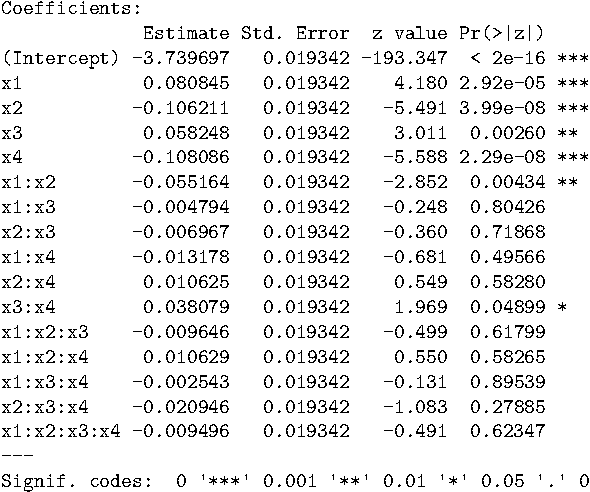
\includegraphics[width=\textwidth]{wk91.pdf}
          \end{figure}
          \begin{itemize}
              \item The $ p $-value for $ \HN $: $ \beta_1=0 $ is $ 2.92\times 10^{-5} $.
              \item The $ p $-value for $ \HN $: $ \beta_2=0 $ is $ 3.99\times 10^{-8} $.
              \item The $ p $-value for $ \HN $: $ \beta_3=0 $ is $ 0.00260 $.
              \item The $ p $-value for $ \HN $: $ \beta_4=0 $ is $ 2.29\times 10^{-8} $.
              \item The $ p $-value for $ \HN $: $ \beta_{12}=0 $ is $ 0.00434 $.
              \item The $ p $-value for $ \HN $: $ \beta_{34}=0 $ is $ 0.04899 $.
          \end{itemize}
    \item We now know which main and interaction effects are significant (i.e., all main effects $ x_1 $:$ x_2 $ and $ x_3 $:$ x_4 $).
          \begin{itemize}
              \item Let's use main and interaction effect plots to help us interpret these effects.
                    \begin{itemize}
                        \item In~\Cref{fig:wk92}, the conversion rate is maximized when the annual fee is low, no account opening fee, and
                              when initial and long-term interest rates are low.
                        \item In~\Cref{fig:wk93}:
                              \begin{itemize}
                                  \item When an account opening fee exists, the effect of the annual fee is less than if there wasn't an account opening fee.
                                  \item As long as long-term interest is low, the effect of initial interest rate is not large.
                              \end{itemize}
                    \end{itemize}
                    \begin{figure}[!htbp]
                        \centering
                        \caption{Main effect plots for the credit card example.}\label{fig:wk92}
                        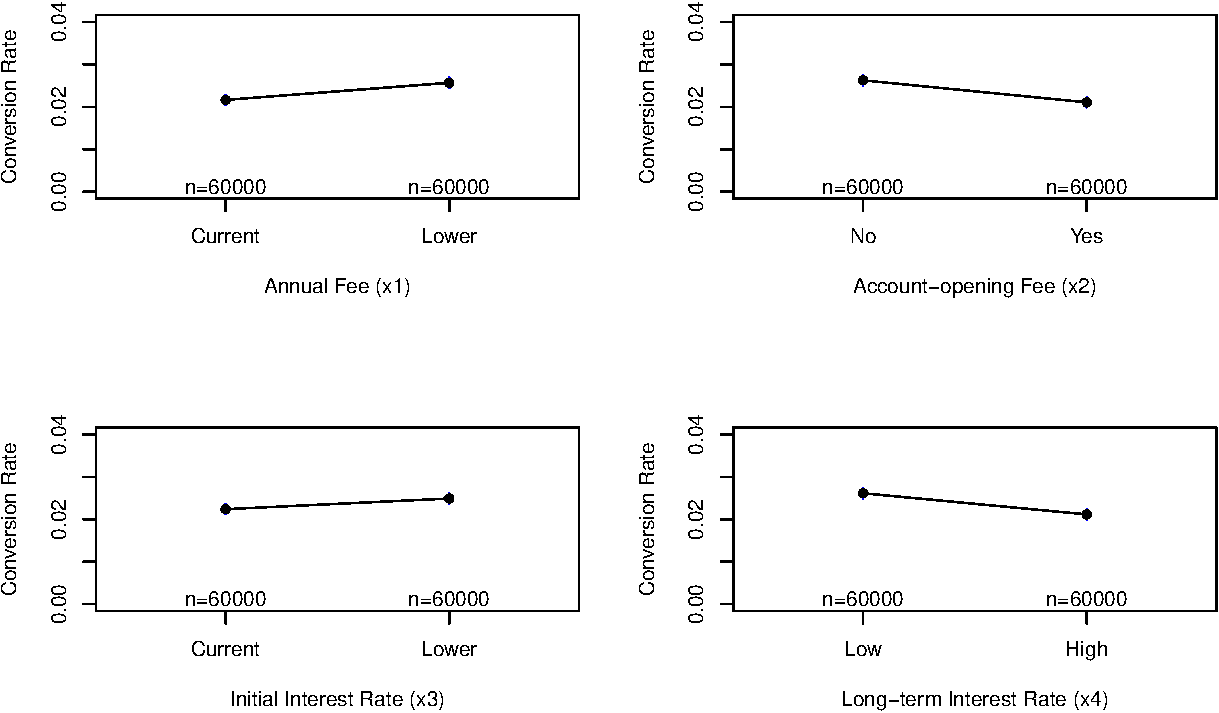
\includegraphics[width=\textwidth]{wk92.pdf}
                    \end{figure}
                    \begin{figure}[!htbp]
                        \centering
                        \caption{Interaction effect plots for the credit card example.}\label{fig:wk93}
                        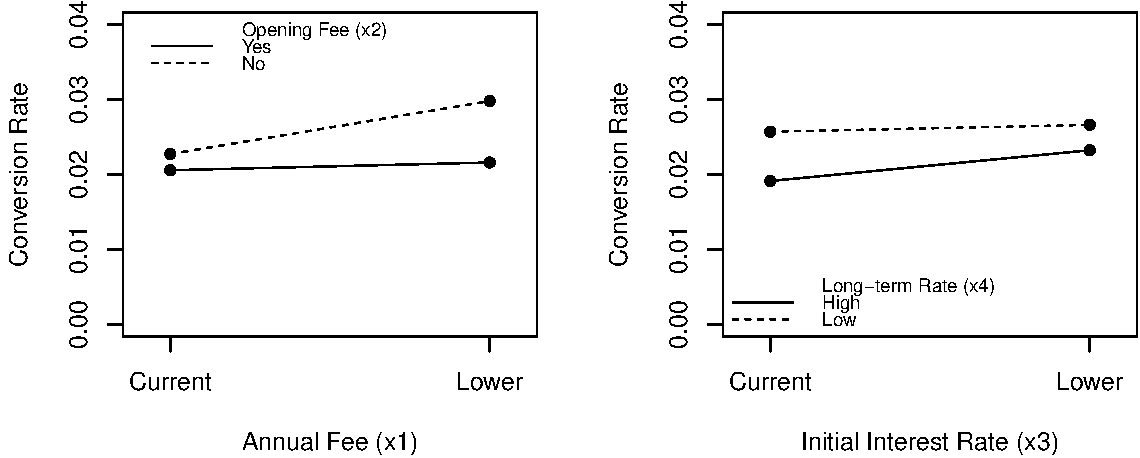
\includegraphics[width=\textwidth]{wk93.pdf}
                    \end{figure}
          \end{itemize}
    \item \href{https://github.com/Hextical/university-notes/blob/master/year-3/semester-3/STAT 430/code/W9/2^4_Factorial_Example.R}{[R Code] \texttt{2\^{}4\_Factorial\_Example}}
\end{itemize}
